\documentclass[sigconf,nonacm]{acmart}

\usepackage{enumitem}
\usepackage{graphicx}
\usepackage{hyperref}
\usepackage{tabularx}
\usepackage{float}
\usepackage[super]{nth}
\usepackage{titlesec}
\usepackage{alltt}
\usepackage{float}

\usepackage[utf8]{inputenc}
%%
%% \BibTeX command to typeset BibTeX logo in the docs
\AtBeginDocument{%
  \providecommand\BibTeX{{%
    \normalfont B\kern-0.5em{\scshape i\kern-0.25em b}\kern-0.8em\TeX}}}
\setlength{\parindent}{0cm}
\setlength{\parskip}{0cm}
\settopmatter{printfolios=true}

\begin{abstract}
This documents the activities and results performed by Group 04 during
\emph{Exercise 2: Reproducibility} of the lecture \emph{188.992 Experiment Design for Data Science}.
\end{abstract}

\renewcommand{\thesection}{\Alph{section})}
\renewcommand{\thesubsection}{(\arabic{subsection})}
\renewcommand{\thesubsubsection}{(\alph{subsubsection})}
\titleformat{\subsubsection}
  {\normalfont\bfseries}{\thesubsubsection}{1em}{}
\titleformat{\paragraph}
  {\normalfont\bfseries\itshape}{}{0em}{}
\begin{document}

%%
%% The "title" command has an optional parameter,
%% allowing the author to define a "short title" to be used in page headers.
\title{Experiment Design, Group 04 -- Reproducibility - Paper 2}

%%
%% The "author" command and its associated commands are used to define
%% the authors and their affiliations.
%% Of note is the shared affiliation of the first two authors, and the
%% "authornote" and "authornotemark" commands
%% used to denote shared contribution to the research.

\author{Helmuth Breitenfellner}
\email{e8725866@student.tuwien.ac.at}
\affiliation{%
}

\author{L\'aszl\'o Kir\'aly}
\email{e9227679@student.tuwien.ac.at}
\affiliation{%
}

\author{Gerald Weber}
\email{e0125536@student.tuwien.ac.at}
\affiliation{%
}

%% A "teaser" image appears between the author and affiliation
%% information and the body of the document, and typically spans the
%% page.
%\begin{teaserfigure}
%  \includegraphics[width=\textwidth]{sampleteaser}
%  \caption{Seattle Mariners at Spring Training, 2010.}
%  \Description{Enjoying the baseball game from the third-base
%  seats. Ichiro Suzuki preparing to bat.}
%  \label{fig:teaser}
%\end{teaserfigure}

%%
%% This command processes the author and affiliation and title
%% information and builds the first part of the formatted document.
\maketitle

\section{Paper selection}

We selected Option 2 - Prediction of music genre across different taxonomies which is based on the paper \textit{MediaEval 2018 AcousticBrainz Genre Task: A Baseline
Combining Deep Feature Embeddings Across Datasets} written by Sergio Oramas, Dmitry Bogdanov and Alastair Porter for the MediaEval conference 2018 in France.
We have choosen the paper because we were curious to reproduce the output of the Neural Network and see what are the problems here in difference to regular Machine Learning papers.


\subsection{Paper Introduction}

The paper is a baseline approach for the MediaEval 2018 AcousticBrainz Genre Task based on a deep neural network.
\textit{The task is focused on content-based musicgenre recognition using genre annotations from multiple sourcesand large-scale music features data available in the AcousticBrainz database} \cite{MediaEval1}.

\subsection{Datasets}

The conference provides a website for the classification task\footnote{\url{https://multimediaeval.github.io/2018-AcousticBrainz-Genre-Task/}, seen on 2020-01-30} which describes the task, the schedule and the dataset on a subpage\footnote{\url{https://multimediaeval.github.io/2018-AcousticBrainz-Genre-Task/data/}, seen on 2020-01-30} in detail.
This subpage contains multiple links:
\begin{itemize}
    \item Zenodo\footnote{\url{https://zenodo.org/record/2553414}, \url{https://zenodo.org/record/2554044}, seen on 2020-01-30} uploaded by Dmitry Bogdanov, Alastair Porter et al.
    \item Google Drive\footnote{\url{https://drive.google.com/drive/folders/0B8wz5KkuLnI3RjFYSFY5TkJVU1U}} containing train/test/validation folders provided by Dmitry Bogdanov and Alastair Porter    
\end{itemize}


The first Zenodo page contains all the required data (lastfm, tag) for the classification task. The second Zenodo page contains restricted access to the AllMusic ground truth, which has been granted after a simple request on the Zenodo page.
The compressed file size is about 47GB.

After decompressing the dataset is structured as followed:
\begin{itemize}
    \item [acousticbrainz-mediaeval-train] 83GB, 1.458.447 files
    \item [acousticbrainz-mediaeval-validation] 18GB, 313.860 files
    \item acousticbrainz-mediaeval-allmusic-train.tsv 260MB (restricted dataset)
    \item acousticbrainz-mediaeval-allmusic-validation.tsv 55MB (restricted dataset)
    \item acousticbrainz-mediaeval-discogs-train.tsv 127MB
    \item acousticbrainz-mediaeval-discogs-validation.tsv 26MB
    \item acousticbrainz-mediaeval-lastfm-train.tsv 62MB
    \item acousticbrainz-mediaeval-lastfm-validation.tsv 14MB
    \item acousticbrainz-mediaeval-tagtraum-train.tsv 59MB
    \item acousticbrainz-mediaeval-tagtraum-validation.tsv 13MB
\end{itemize}
Total size of the extracted files: 102GB

The folders contains subfolders ranging from 00-ff containing JSON files. These files contains precomputed Audio features extracted with Essentia\footnote{} from the community-built AcousticBrainz database.

The .tsv files contains features in the format:
recordingmbid   releasegroupmbid        genre1  genre2  genre3  genre4  genre5  genre6  genre7  genre8  genre9   genre10 genre11 genre12 genre13 genre14 genre15 genre16 genre17 genre18 genre19 genre20 genre21 genre22  genre23 genre24 genre25 genre26 genre27 genre28 genre29 genre30 genre31 genre32 genre33 genre34 genre35  genre36 genre37 genre38 genre39 genre40

The field \textit{recordingmbid} is the MusicBrainz identifier of the particular recording, whereas \textit{releasegroupmbid} is a MusicBrainz identifier of a release group (an album, single, or compilation) that it belongs to. The related genres and subgenres are encoded into the columns \textit{genre1-genre40}.
For each recordingmbid there exists a file the \textit{acousticbrainz-mediaeval-train} folder.



\section{Paper - Reproduction}

The authors of the paper provided a link to a Github repository\footnote{\url{https://github.com/MTG/acousticbrainz-mediaeval-baselines}, seen on 2020-01-30} which contains a data-preparation folder and a link to another repository\footnote{\url{https://github.com/sergiooramas/tartarus/tree/b214f66dd4e61e83edc45ffc5c280efe7318a1b6}, seen on 2020-01-30}. 
This linked repository contains three experiments written by Oramas et al. . Based on the description of the experiments and on the number of features described in the paper (2669) we could identify experiment 3: \textit{TISMIR Experiments (Single\-label Classification)}\footnote{denoted in the run\_experiments.py as \textit{ISMIR 2019 Experiments (Baseline for AcousticBrainz Genre Dataset Classification)}} as the baseline approach.

With this information we inspected the \textit{data\-preparation/create\_h5.py} file to find out how to prepare the data. The existing file \textit{data-preparation/create\_h5.py} requires some \textit{.features.clean.std.csv} and \textit{.clean.std.csv} as well as \textit{.genres.csv} as input. None of them is available in the dataset.

Tries to contact the main author via two mail addresses (soramas@pandora.com, sergio.oramas@upf.edu) were not successful.


\section{Reproducing \#2 - A new hope} 

Some online research led us to a recently created Github repository\footnote{\url{https://github.com/nikuya3/acousticbrainz-mediaeval-baseline}, seen on 2020-01-30} which deals with the same paper. Additionally it has a preprocessing step included. Naturally, we cloned the repository and started \textit{}


\subsection{Datasets}

\subsection{Preprocessing}
  \begin{figure}
    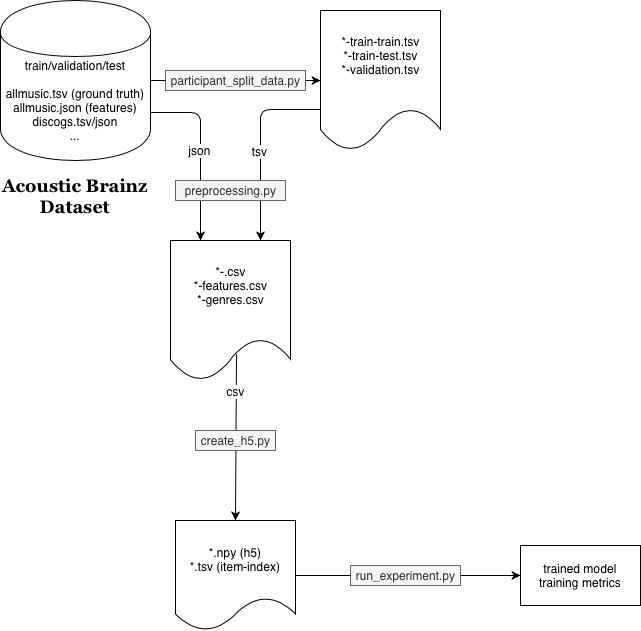
\includegraphics[width=\linewidth]{Preprocess-Data.png}
    \caption{Preprocessing Data.}
    \label{fig:preprocess}
  \end{figure}

  \begin{itemize}
    \item preprocessing.py python3
    \item participant\_split\_data.py
    \item create\_h5.py python2 with h5py
  \end{itemize}

  Problems:
  \begin{itemize}
    \item TypeError: No conversion path for dtype: dtype('<U38') https://github.com/h5py/h5py/issues/1131 -> solved with using python2
  \end{itemize}

\subsection{Train}

\begin{itemize}
  \item run\_experiment python3
\end{itemize}

Problems:
\begin{itemize}
  \item ValueError: Error when checking target: expected dense\_5 to have shape (766,) but got array with shape (1,)
\end{itemize}

\subsection{Sources}

\subsection{Doing}




\bibliography{bibliography}
\bibliographystyle{alpha}

\end{document}
\endinput
